% ==================================================
%   LaTeX sablon - Dokumentáció/HF/Beadandó
%
%   Készítette:        Agócs Norbert
%   Dátum:             2025.09.01.
%   Utolsó frissítés:  2025.10.01.
%
%   License: MIT
% ==================================================

% --------------------------------------------------
% Fájl: main.tex
% --------------------------------------------------

% Dokumentum konfiguráció
\documentclass[fleqn,12pt]{article}

% --------------------------------------------------
% Dokumentum adatok
% --------------------------------------------------

% Intézmény és kar
\newcommand\INTEZMENY{Budapesti Műszaki és Gazdaságtudományi Egyetem}
\newcommand\KAR{Gépészmérnöki Kar}
\newcommand\LOGO{bme-logo.jpg} % logo fájl neve a figures mappában

% Dokumentum adatok
% TODO
\newcommand\CIM{\LaTeX{} dokumentáció tutorial}
\newcommand\DATUM{2025/26/1}
\newcommand\NEV{Agócs Norbert}
\newcommand\NEPTUN{PhD hallgató}
\newcommand\EMAIL{nagocs@mm.bme.hu}
\newcommand\TANTARGY{Tantárgy}
\newcommand\TANTARGYKOD{BMEGE\dots}

% --------------------------------------------------
% Preambulum és egyéni parancsok betöltése
% --------------------------------------------------

% --------------------------------------------------
% Fájl: 00_preambulum.tex
% --------------------------------------------------

% --------------------------------------------------
% Packagek
% --------------------------------------------------

% Dokumentum konfiguráció
\usepackage[hungarian]{babel} % dokumentum nyelvi beállítása
\usepackage[utf8]{inputenc} % bemeneti betűkódolás (ékezetes karakterek)
\usepackage[T1]{fontenc} % kimeneti betűkódolás (ékezetes karakterek)
\usepackage{lmodern} % bővített karakterkészlet az ékezetekhez
\usepackage{geometry} % dokumentum margók és oldalbeállítások
\usepackage{hyperref} % hivatkozások és linkek
\usepackage[backend=biber,style=numeric,sorting=none]{biblatex} % irodalomjegyzék

% Ábrák, grafikák
\usepackage{graphicx} % klépek beillesztése és méretezése
\usepackage{float} % ábrák és táblázatok elhelyezésének pontos szabályozása
\usepackage{caption} % képaláírások formázása
\usepackage{tikz} % vektorgrafikák, ábrák rajzolása LaTeX-ben
\usepackage{xcolor} % színek kezelése
\usepackage{pdfpages} % teljes PDF-oldalak beillesztése a dokumentumba

% Matematikai és fizikai írásmód
\usepackage{amsmath,amsthm,amsfonts,amssymb,amscd} % matematikai környezetek és szimbólumok
\usepackage{mathtools} % kiegészítő matematikai eszközök az amsmath-hoz
\usepackage{siunitx} % SI mértékegységek helyes jelölése

% Fejléc, lábléc
\usepackage{fancyhdr} % egyedi fejléc és lábléc készítése
\usepackage{lastpage} % az utolsó oldal sorszámának hivatkozása

% Dokumentumtagolás
\usepackage{titlesec} % címsorok formázásának testreszabása
\usepackage{csquotes} % idézetek helyes formázása (nyelvspecifikus)
\usepackage{booktabs} % szép, tipográfiailag helyes táblázatok készítése


% --------------------------------------------------
% Dokumentum beállítások
% --------------------------------------------------

% Dokumentum formátum
\geometry{a4paper,total={170mm,240mm},left=20mm,top=30mm} % oldalbeállítások: A4, margók méretezése
\setlength\parindent{0pt} % bekezdések behúzásának kikapcsolása

% Fejléc, lábléc beállítása
\pagestyle{fancy} % fancyhdr csomag stílus használata
\renewcommand{\headrulewidth}{0.4pt} % fejléc vonalvastagsága
\renewcommand{\footrulewidth}{0.4pt} % lábléc vonalvastagsága
\headheight 1.5em % fejléc magasságának beállítása
\rhead{\NEV{}, \NEPTUN{}} % jobb felső sarok
\chead{} % középső fejléc
\lhead{\TANTARGYKOD{}, \TANTARGY{}} % bal felső sarok
\lfoot{} % bal alsó sarok
\cfoot{} % középső lábléc
\rfoot{\small\thepage\ / \pageref{LastPage}} % jobb alsó sarok
\headsep 1.5em % fejléc és szöveg közötti távolság

% Hyperref beállítások - PDF megjelenítés
\hypersetup{
    colorlinks=true, % színes linkek
    linkcolor=blue, % belső hivatkozások színe
    urlcolor=cyan, % URL hivatkozások színe
    pdftitle={\CIM{}}, % PDF cím
    pdfauthor={\NEV{}}, % PDF szerző
    pdfsubject={\TANTARGY{} (\TANTARGYKOD{})}, % PDF tárgy
    bookmarksopen=true, % könyvjelzők alapból nyitva
    bookmarksnumbered=true, % könyvjelzők számozása
    pdfpagemode=UseOutlines % könyvjelzők megjelenítése PDF olvasóban
}

% Irodalomjegyék beállítása
\addbibresource{contents/literature.bib} % irodalomjegyzék forrásfájl

% Számozások beállítása fejezetenként
% \numberwithin{equation}{section} % egyenletek számozása fejezetenként
% \numberwithin{figure}{section} % ábrák számozása fejezetenként
% \numberwithin{table}{section} % táblázatok számozása fejezetenként

% Táblázat formátum beállítása - Függőlegesen középre igazított szöveg
\newcolumntype{L}[1]{>{\raggedright\let\newline\\\arraybackslash\hspace{0pt}}m{#1}} % balra zárt
\newcolumntype{C}[1]{>{\centering\let\newline\\\arraybackslash\hspace{0pt}}m{#1}} % középre zárt
\newcolumntype{R}[1]{>{\raggedleft\let\newline\\\arraybackslash\hspace{0pt}}m{#1}} % jobbra zárt
\renewcommand{\arraystretch}{1.25} % táblázatok sormagassága

% Mértékegységek formátuma
\sisetup{exponent-product = \cdot, per-mode=fraction} % SI jelölések

% Tikz
\usetikzlibrary{math} % matematikai számítások Tikz-ben
\usetikzlibrary{calc} % geometriai számítások (pl. koordináták)
\usetikzlibrary{angles} % szögjelölések rajzolása
\usetikzlibrary{quotes} % címkék és feliratok egyszerű kezelése
\usetikzlibrary{arrows.meta} % nyílstílusok




% --------------------------------------------------
% Fájl: 01_commands.tex
% --------------------------------------------------

% --------------------------------------------------
% Matematikai parancsok
% --------------------------------------------------

% Általános matematikai parancsok
\renewcommand{\d}[1]{\mathrm{d}#1} % differenciál jel
\renewcommand{\vec}[1]{\mathbf{#1}} % vektor jelölés
\newcommand{\norm}[1]{\left\lVert #1 \right\rVert} % norma
\newcommand{\abs}[1]{\left\lvert #1 \right\rvert} % abszolút érték

% Lineár algebrai műveletek
\DeclareMathOperator{\rank}{rank} % rang
\DeclareMathOperator{\tr}{tr} % nyom (trace)
\DeclareMathOperator{\diag}{diag} % diagonális mátrix

% Vektoranalízis műveletek
\DeclareMathOperator{\grad}{\mathbf{grad}} % grad
\DeclareMathOperator{\rot}{\mathbf{rot}} % rot
\DeclareMathOperator{\diverg}{\mathbf{div}} % div
\DeclareMathOperator{\laplace}{\Delta} % Laplace-operátor

% Egyéb műveletek
\newcommand{\eval}[2]{\left. #1 \right|_{#2}} % kifejezés kiértékelése

% --------------------------------------------------
% Egyéb parancsok
% --------------------------------------------------

\newcommand*\circled[1]{\begin{tikzpicture}[baseline=(C.base)] \node[draw,circle,inner sep=2pt](C) {#1}; \end{tikzpicture}} % karikázás

% ==================================================
% Dokumentum kezdete
% ==================================================
\begin{document}

% Címlap és tartalomjegyzék
%-------------------------------------------------------------------
% Fájl: 01_title.tex
%-------------------------------------------------------------------

% Oldal beállítások
\frenchspacing
\thispagestyle{empty} % Ne legyen header

%-------------------------------------------------------------------
% Fejléc
\begin{center}
   \includegraphics[width=0.35\linewidth]{figures/bme-logo.jpg} \\
   \vskip 0.5em
   \textsc{Budapesti Műszaki és Gazdaságtudományi Egyetem} \\
   \textsc{Gépészmérnöki Kar}
\end{center}

%-------------------------------------------------------------------
% Elválasztóvonal
\begin{center}
   \noindent\rule{0.99\textwidth}{0.25pt}
\end{center}

%-------------------------------------------------------------------
% Cím
\begin{center}
   \LARGE{\textbf{\CIM}} \\
   \vskip 0.5em
   \large{\TANTARGY{} (\TANTARGYKOD{})} \\
   \vskip 0.25em
   \large{\NEV{} (\url{\EMAIL})} \\
   \vskip 0.25em
   \DATUM{}
\end{center}

%-------------------------------------------------------------------
% Elválasztóvonal
\begin{center}
   \noindent\rule{0.99\textwidth}{0.25pt}
\end{center}
%\includepdf[pages=-]{contents/feladatlap.pdf} % feladatlap beszúrása, ha szükséges
% --------------------------------------------------
% Fájl: 02_contentpage.tex
% --------------------------------------------------

% --------------------------------------------------
% Tartalomjegyzék 
% --------------------------------------------------

\tableofcontents % tartalomjegyzék kiírása
\newpage % új oldal kezdése a tartalomjegyzék után
\setcounter{page}{1} % az oldalszámozás újraindítása 1-től

% --------------------------------------------------
% 0. fejezet
% --------------------------------------------------
\section{A jelen dokumentum célja}

    \emph{A jelen dokumentum egy tutorialként szolgál a dokumentációk, házi feladatok és egyéb beadandók \LaTeX-ben történő elkészítéséhez. Célja, hogy bemutassa a sablon alkalmazását, valamint azokat az alapvető \LaTeX{} parancsokat, amelyek elsajátításával könnyen és egységes formátumban készíthető el a szükséges dokumentáció.}

    \vspace{0.5em}
    \textcolor{red}{A dokumentum tanulmányozásakor célszerű a generált \texttt{tutorial.pdf} fájlt és a hozzá tartozó \texttt{tutorial.tex} forrásfájlt egymással párhuzamosan áttekinteni, így a kód és annak eredménye közvetlenül összevethető.}


% --------------------------------------------------
% 1. fejezet
% --------------------------------------------------
\section{\LaTeX{} tutorial}

    A \LaTeX{} egy széles körben használt dokumentumszerkesztő keretrendszer, amely különösen alkalmas tudományos és műszaki dokumentumok készítésére. A \LaTeX{} lehetővé teszi a felhasználók számára, hogy a dokumentumok tartalmára összpontosítsanak, miközben a formázást és a megjelenést a rendszer globálisan kezeli.

    \vspace{0.5em}
    A \LaTeX{} használata kezdetben bonyolultnak tűnhet, de a sablonok és a példák segítségével gyorsan elsajátítható. A következőkben egy rövid útmutatót találhatsz a legfontosabb \LaTeX{} funkciókról és azok használatáról.

    \subsection{Matematikai szimbólumok}

        A \LaTeX{} egyik legfontosabb és legtöbbet használt funkciója a matematikai képletek és szimbólumok írása. A matematikai képleteket és szimbólumokat matematikai módban érhetjük el. A matematikai módba többféleképpen lehet belépni:
        \begin{itemize}
            \item \texttt{\$ ... \$} --- egy soron belüli (inline) képlet,
            \item \texttt{\$\$ ... \$\$} --- külön sorba helyezett, középre igazított képlet.
        \end{itemize}

       A legalapvetőbb szimbólumok és jelölések a következők:
        \begin{itemize}
            \item Skalár változók: $x$, $y$, $z$, $a$, $b$, $c$
            \item Vektorok, mátrixok: $\vec{v}$, $\vec{u}$, $\vec{w}$, $\mathbf{A}$, $\mathbf{B}$
            \item Görög betűk: $\alpha$, $\beta$, $\gamma$, $\pi$, $\lambda$, $\Omega$
            \item Függvények: $\sin(x)$, $\cos(x)$, $\tan(x)$, $\log(x)$, $\exp(x)$, $\mathrm{e}^{x}$, $\sqrt{x}$, $\sqrt[3]{y}$
            \item Indexek és hatványok: $x_i$, $x^2$, $a_{ij}$
            \item Törtek: $\frac{a}{b}$
            \item Szummázás: $\sum_{i=1}^{n} i$
            \item Határérték: $\lim_{x \to 0} \frac{\sin x}{x}$
            \item Deriválás: $\frac{\mathrm{d}y}{\mathrm{d}x}$, $\frac{\partial z}{\partial x}$
            \item Integrálás: $\int_{0}^{1} x^2 \,\mathrm{d}x $, $\iint_{D} f(x,y) \,\mathrm{d}x \,\mathrm{d}y$
        \end{itemize}

    \subsection{Vektorok, mátrixok}

        A vektorokat nyomtatásban vastagon szedett kis betűvel jelöljük, például $\mathbf{v}$, $\mathbf{u}$, $\mathbf{w}$. A mátrixokat szintén vastagon szedett nagy betűkkel jelöljük, például $\mathbf{A}$, $\mathbf{B}$. A vektorokat és mátrixokat a \texttt{bmatrix}, \texttt{pmatrix} környezettel lehet definiálni:
        \begin{align}
            \mathbf{A} &=
            \begin{bmatrix}
                1 & 2 & 3 \\
                4 & 5 & 6 \\
                7 & 8 & 9
            \end{bmatrix}, &
            \mathbf{a} &=
            \begin{bmatrix}
                1 \\
                2 \\
                3
            \end{bmatrix} &
            \mathbf{x} &=
            \begin{bmatrix}
                x_1 \\
                x_2 \\
                x_3
            \end{bmatrix}.
        \end{align}

    \subsection{Egyenletek}

        Az egyenleteket mindig külön sorban szokás megjeleníteni, balra vagy középre igazítva, és a jobb oldalon számozással ellátva. A \LaTeX{} ehhez több környezetet biztosít:
        \begin{itemize}
            \item \texttt{\textbackslash begin\{equation\} ... \textbackslash end\{equation\}} --- egy soros, számozott egyenlet,
            \item \texttt{\textbackslash begin\{align\} ... \textbackslash end\{align\}} --- több soros, számozott egyenletek, igazítva,
            \item \texttt{\textbackslash begin\{multline\} ... \textbackslash end\{multline\}} --- hosszabb egyenlet több sorba tördelve,
            \item \texttt{\textbackslash begin\{gather\} ... \textbackslash end\{gather\}} --- több független egyenlet, középre igazítva.
        \end{itemize}

        Az egyenletek a mondat szerves részei, így a megfelelő írásjeleket az egyenlet után is ki kell tenni. Például a nyomaték redukciós képlet a következőképpen írható fel:
        \begin{equation}
            \vec{M}_A = \vec{M}_B + \vec{r}_{BA} \times \vec{F}. \label{eq:moment_reduction}
        \end{equation}
        Az egyenletben szereplő változókat, mennyiségeket és konstansokat a fő szöveg részeként kell definiálni. Ezt többféleképpen is megtehetjük.

        \begin{enumerate}
            \item \emph{Az egyenlet után közvetlenül}: \dots ahol $\vec{M}_A$ az $A$ pontbeli nyomatékvektor, $\vec{M}_B$ a $B$ pontbeli nyomatékvektor, $\vec{r}_{BA}$ a $B$-ből $A$-ba mutató helyvektor, és $\vec{F}$ a ható erővektor. 
            \item \emph{Hivatkozással}: a \eqref{eq:moment_reduction} egyenletben szereplő $\vec{M}_A$ az $A$ pontbeli nyomatékvektor, $\vec{M}_B$ a $B$ pontbeli nyomatékvektor, $\vec{r}_{BA}$ a $B$-ből $A$-ba mutató helyvektor, és $\vec{F}$ a ható erővektor.
            \item \emph{Felsorolásszerűen}: a \eqref{eq:moment_reduction} egyenletben szereplő mennyiségek jelentése a következők:
                \begin{align*}
                    \vec{M}_A &\quad \text{az $A$ pontbeli nyomatékvektor}, \\
                    \vec{M}_B &\quad \text{a $B$ pontbeli nyomatékvektor}, \\
                    \vec{r}_{BA} &\quad \text{a $B$-ből $A$-ba mutató helyvektor}, \\
                    \vec{F} &\quad \text{a ható erővektor}.
                \end{align*}
        \end{enumerate}

    Ha egy egyenlet olyan hosszú, hogy túlnyúlik az oldalszélességen, akkor célszerű több sorban tördelni. (Ugyanakkor érdemes kerülni a túlzottan hosszú kifejezéseket.) Például a következő differenciálegyenlet írható fel egy hajlított gerenda lehajlására:
    \begin{multline}
        EI \, \frac{\mathrm{d}^4 w(x)}{\mathrm{d}x^4} 
        + c_1 \frac{\mathrm{d}^3 w(x)}{\mathrm{d}x^3}
        + c_2 \frac{\mathrm{d}^2 w(x)}{\mathrm{d}x^2}
        + c_3 \frac{\mathrm{d} w(x)}{\mathrm{d}x}
        + c_4 w(x) \\
        = q_0 \sin\!\left(\frac{\pi x}{L}\right)
        + q_1 \cos\!\left(\frac{2\pi x}{L}\right)
        + q_2 e^{-\alpha x} \cos(\beta x)
        + q_3 x^2
        + q_4 \ln(1+x),
    \end{multline}
    ahol $EI$ a hajlítómerevség, $w(x)$ a lehajlás, $c_i$ konstans tényezők, $q_i$ terhelési paraméterek, $L$ a gerenda hossza, $\alpha$ és $\beta$ pedig az exponenciális-ciklikus terhelés paraméterei.    

    \subsection{Mértékegységek és mennyiségek}

        A fizikai mennyiségek mértékegységeit mindig álló betűvel kell írni, például $\mathrm{N}$, $\mathrm{m}$, $\mathrm{s}$. A mérőszám és a mértékegység közé nem törhető szóközt kell tenni (LaTeX-ben: \texttt{\~}), hogy a szám és a mértékegység ne váljon szét a sor végén. Például:
        $$
        5~\mathrm{m}, \quad 10~\mathrm{s}, \quad 20~\mathrm{N}.
        $$
        Kivételt képez a százalék, ahol a szám és a jel közé nem kerül szóköz: $50\%$.

        \vspace{1em}
        A \LaTeX{}-ben a mértékegységek és számok egységes, szabványos formázására a \texttt{siunitx} csomag a legkényelmesebb megoldás. Ez a csomag automatikusan biztosítja a helyes tipográfiát, a nem törhető szóközt, a tizedesjel formátumát és az SI-egységek helyes megjelenítését. Néhány példa:
        \begin{itemize}
            \item \verb|\qty{5}{m}| → \qty{5}{m}
            \item \verb|\qty{9.81}{m/s^2}| → \qty{9.81}{m/s^2}
            \item \verb|\qty{1.23e4}{J}| → \qty{1.23e4}{J}
            \item \verb|\num{12345.6789}| → \num{12345.6789}
        \end{itemize}

    \subsection{Táblázatok}

        A táblázatok létrehozásához a \texttt{table} és \texttt{tabular} környezeteket használjuk. A táblázatok mindig tartalmazzanak sorszámot és címet, hogy hivatkozhassunk rájuk a szövegben. A táblázatok címét mindig a táblázat felett kell elhelyezni. Például:
        \begin{table}[htb!]
            \centering
            \begin{tabular}{C{2cm}C{3cm}C{3cm}}
                \toprule
                \textbf{Jelölés} & \textbf{Mértékegység} & \textbf{Érték} \\
                \midrule
                $a$ & \unit{mm} & 6 \\
                $b$ & \unit{mm} & 7 \\
                $c$ & \unit{mm} & 545 \\
                $d$ & \unit{mm} & 545 \\
                \midrule
                $F_1$ & \unit{kN} & 7 \\
                $F_2$ & \unit{kN} & 6 \\
                $M_1$ & \unit{kNm} & 1 \\
                \bottomrule
            \end{tabular}
            \caption{A számításhoz megadott adatok.}
            \label{table:adatok}
        \end{table}

        A fenti táblázatra a következőképpen hivatkozhatunk a szövegbe: \aref{table:adatok}. táblázatban szereplő adatok alapján elmondható, hogy \dots A táblázatok készítéséhez a \texttt{booktabs} csomag használata erősen ajánlott, mivel sokkal esztétikusabbá teszi a táblázatokat.
    
    \newpage
    \subsection{Ábrák}

        Az ábrák beillesztéséhez a \texttt{figure} környezetet használjuk. Az ábráknak is legyen sorszámuk és címük, hogy hivatkozhassunk rájuk a szövegben. Az ábrák címét mindig az ábra alatt kell elhelyezni. Például:
        \begin{figure}[htb!]
            \centering
            \includegraphics[width=0.75\linewidth]{figures/sample-fig.pdf}
            \caption{Egy minta ábra.}
            \label{fig:sample_figure}
        \end{figure}

        A fenti ábrára a következőképpen hivatkozhatunk a szövegbe: \aref{fig:sample_figure}. ábra mutatja be a minta ábrát. Az ábrák készítéséhez használhatunk külső programokat (pl. Python, MATLAB, Excel), vagy \LaTeX-ben is rajzolhatunk ábrákat a \texttt{Ti\emph{k}Z} csomag segítségével.

    \subsection{Ti\emph{k}Z}

        A \texttt{Ti\emph{k}Z} egy grafikai csomag \LaTeX-hez, amely lehetővé teszi vektoros ábrák készítését közvetlenül a dokumentumban. A \texttt{Ti\emph{k}Z} segítségével bármilyen ábrát létrehozhatunk. Például egy egyszerű mechanikai modell rajzolása a következőképpen történik:
        \begin{figure}[htb!]
            \centering
            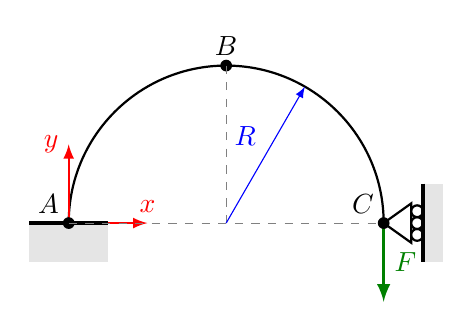
\begin{tikzpicture}[
    % --- Saját stílusok definiálása ---
    vec/.style = {color=#1,very thick,-latex}, % vektor stílus, nyíllal
    link/.style = {color=#1, thick},           % vonal stílus
    point/.style = {circle,fill=black,inner sep = 1.5pt}, % csomópontok
    guide/.style = {color=#1,thin},            % segédvonal stílus
    coordSys/.style = {color=#1, thick,-latex} % koordinátarendszer nyilai
    ]

    % --- Paraméterek definiálása ---
    \def\r{2}        % sugár
    \def\phi{60}     % szög (fokban)

    % --- Koordináták megadása ---
    \coordinate (A) at (0,0);                            % A pont (origó)
    \coordinate (B) at (\r,\r);                          % B pont
    \coordinate (C) at (2*\r,0);                         % C pont
    \coordinate (O) at (\r,0);                           % O középpont
    \coordinate (P) at ({\r+\r*cos(\phi)},{\r*sin(\phi)}); % P pont (szög szerint)

    % --- Test (félkörív) kirajzolása ---
    \draw[link={black}] (A) arc (180:0:\r);

    % --- Erő vektora ---
    \draw[vec={green!50!black}] (C) -- node[midway, right] {$F$} +(0,-1);

    % --- Koordináta-rendszer kirajzolása ---
    \draw[coordSys={red}] (A) -- +(0,1) node[left] {$y$};  % y tengely
    \draw[coordSys={red}] (A) -- +(1,0) node[above] {$x$}; % x tengely

    % --- Támasz (háromszög és görgők) C pontnál ---
    \draw[link={black}, fill=white] (C) -- ($(C)+(0.35, 0.25)$) -- ($(C)+(0.35, -0.25)$) -- cycle;
    \foreach \i in {-0.15, 0, 0.15} {
        \draw[link={black}, fill=white] ($(C)+(0.425, \i)$) circle (0.075);
    }

    % --- Talaj ábrázolása A és C pont alatt ---
    \fill[gray!20!white] ($(A)+(-0.5,0)$) rectangle ($(A)+(0.5,-0.5)$);
    \draw[black,very thick] ($(A)+(-0.5,0)$) -- ($(A)+(0.5,0)$);
    \fill[gray!20!white] ($(C)+(0.5,0.5)$) rectangle ($(C)+(0.75,-0.5)$);
    \draw[black,very thick] ($(C)+(0.5,0.5)$) -- ($(C)+(0.5,-0.5)$);
    
    % --- Csomópontok megrajzolása ---
    \node[point] at (A) {};
    \node[point] at (B) {};
    \node[point] at (C) {};
    \node[above left] at (A) {$A$};
    \node[above] at (B) {$B$};
    \node[above left] at (C) {$C$};

    % --- Segédvonalak és sugár vektora ---
    \draw[guide={gray}, dashed] (A) -- (C);      % A és C közötti szaggatott vonal
    \draw[guide={gray}, dashed] (B) -- +(0,-\r); % B-ből függőleges segédvonal
    \draw[guide={blue}, -latex] (O) -- node[above left] {$R$} (P); % sugár vektor
\end{tikzpicture}

            \caption{Egy egyszerű mechanikai modell TikZ ábrája.}
            \label{fig:tikz_example}
        \end{figure}

        A fenti ábrára a következőképpen hivatkozhatunk a szövegbe: \aref{fig:tikz_example}. ábra mutatja be a Ti\emph{k}Z használatát egy mechanikai modell rajzolására. A TikZ ábrákat külön fájlban is tárolhatjuk, és a \texttt{\textbackslash input\{...\}} paranccsal illeszthetjük be a dokumentumba.

    \subsection{Hivatkozások és irodalomjegyzék}

        A dokumentumban található különféle egyenletekre, táblázatokra és ábrákra a \texttt{\textbackslash label\{...\}} és \texttt{\textbackslash ref\{...\}} parancsok segítségével hivatkozhatunk. Például a \eqref{eq:moment_reduction} egyenletben látható a nyomaték redukciós képlete.

        \vspace{1em}
        Az irodalomjegyzék létrehozásához a \texttt{biblatex} csomagot használjuk. Az irodalomjegyzékhez egy külön \texttt{.bib} fájlt kell létrehozni, amelyben a hivatkozásokat tároljuk a megadott formátumban.
        Példa egy hivatkozásra a \texttt{literature.bib} fájlban:
        \begin{verbatim}
        @book{latex2e,
            author = {Leslie Lamport},
            year = {1994},
            title = {{\LaTeX}: a Document Preparation System},
            publisher = {Addison Wesley},
            address = {Massachusetts},
            edition = {2}
        }
        \end{verbatim}

        A hivatkozások beszúrásához a \texttt{\textbackslash cite\{...\}} parancsot használjuk, ahol a \texttt{literature.bib} fájlban definiált hivatkozás neve szerepel. Például: \verb|\cite{latex2e}| \cite{latex2e}. 
        
        \vspace{1em}
        Az irodalomjegyzék automatikusan generálódik a dokumentum végén, és a hivatkozások formátuma a választott stílustól függ. A sablonban a \texttt{numeric} stílus van beállítva, de más stílusok is használhatók, például \texttt{authoryear}, \texttt{alphabetic}, stb.

    \subsection{További források}

        A \LaTeX{} használatáról és a különböző csomagokról számos segédlet, online forrás és dokumentáció érhető el. A következő források hasznosak lehetnek a \LaTeX{} elsajátításához:
        \begin{itemize}
            \item \url{https://www.latex-project.org/} --- A hivatalos \LaTeX{} projekt oldala.
            \item \url{https://ctan.org/} --- A \LaTeX{} csomagok dokumentációi.
            \item \url{https://www.overleaf.com/learn} --- Overleaf dokumentáció és oktatóanyagok.
            \item \url{https://tex.stackexchange.com/} --- Közösségi fórum a \LaTeX{} felhasználók számára
            \item \url{https://wch.github.io/latexsheet/} --- \LaTeX{} cheatsheet
            \item \url{https://en.wikibooks.org/wiki/LaTeX} --- Wikikönyv \LaTeX{}-ről
        \end{itemize}

        A \LaTeX{} használatának elsajátításához sokat kell gyakorolni, de a sablon és a fenti források segítségével gyorsan elindulhatsz a dokumentumkészítés útján. 

% --------------------------------------------------
% 2. fejezet
% --------------------------------------------------

\section{A sablon használata}

   A sablon célja, hogy egységes keretet adjon a BME Gépészmérnöki Karán készítendő dokumentációk, házi feladatok és beadandók elkészítéséhez. Előre definiált formázási és szerkezeti elemeket tartalmaz, valamint példákat a gyakran használt \LaTeX{} funkciókra. 

    \vspace{0.5em}
    \textcolor{red}{A sablon használata nem kötelező, ugyanakkor jelentősen megkönnyíti a dokumentumkészítést azáltal, hogy egy kész struktúrát és stílust biztosít.}

    \subsection{Dokumentum felépítése}

        A dokumentum fő részei külön \texttt{.tex} fájlokra vannak bontva annak érdekében, hogy a sablon átláthatóbb és a szövegszerkesztés egyszerűbb legyen.  A központi szerepet a \texttt{main.tex} fájl tölti be, amely tartalmazza a dokumentum alapszerkezetét, és innen hivatkozunk a további részekre. 

        \vspace{0.5em}
        \textcolor{red}{A szövegszerkesztés során mindig a \texttt{main.tex} fájlt kell megnyitni és szerkeszteni, mivel ez a fájl tartalmazza a dokumentum teljes lényegi tartalmát.}
        
        \vspace{1em}
        A fájlok logikusan elkülönítve, külön mappákban találhatók:
        \begin{itemize}
            \item \texttt{settings} — a dokumentum beállításait és az egyéni parancsokat tartalmazó fájlok,
            \item \texttt{contents} — a dokumentum tartalmi elemeit tartalmazó fájlok,
            \item \texttt{figures} — a dokumentumban használt ábrák és képek gyűjtőhelye.
        \end{itemize}

        A legfontosabb fájlok és feladataik a következők:
        \begin{itemize}
            \item \texttt{settings/00\_preambulum.tex} — azokat a csomagokat és beállításokat tartalmazza, amelyek az egész dokumentumra érvényesek. \emph{Nem szükséges módosítani.}
            \item \texttt{settings/01\_commands.tex} — az egyéni parancsok gyűjteménye, ahová a gyakran használt, saját definiálású parancsokat célszerű beírni. 
            \item \texttt{contents/01\_title.tex} — a címlap összeállítására szolgál. \emph{Ezt a fájlt általában nem szükséges módosítani, a dokumentum adatai a preambulumban adhatók meg.}
            \item \texttt{contents/02\_contentpage.tex} — a tartalomjegyzék létrehozásáért felel. \emph{Ezt a fájlt sem kell szerkeszteni, mivel a tartalomjegyzék automatikusan generálódik.}
            \item \texttt{contents/03\_bib.tex} — az irodalomjegyzék előállítását végzi. \emph{Szintén nem igényel kézi módosítást, az irodalomjegyzék automatikusan épül fel a hivatkozások alapján.}
            \item \texttt{contents/literature.bib} — a hivatkozások tárolására szolgáló fájl, amit a \texttt{biblatex} csomag használ az irodalomjegyzék összeállításához.
        \end{itemize}

    \subsection{Dokumentum használata}

        A sablon használatához elegendő a \texttt{main.tex} fájlt szerkeszteni, a többi fájl előre definiált szerkezeti és formázási elemeket tartalmaz, amelyek módosítására általában nincs szükség. A szövegszerkesztéskor a következő lépéseket érdemes követni:

        \begin{enumerate}
            \item \textbf{Dokumentum adatok kitöltése.}  A \texttt{main.tex} elején található parancsokban kell megadni az alapvető adatokat:
            \begin{itemize}
                \item \verb|\CIM| — a dokumentum címe,
                \item \verb|\DATUM| — a beadás dátuma vagy félév megjelölése,
                \item \verb|\NEV| és \verb|\NEPTUN| — a hallgató neve és Neptun-kódja,
                \item \verb|\EMAIL| — e-mail cím,
                \item \verb|\TANTARGY| és \verb|\TANTARGYKOD| — a tantárgy neve és kódja,
                \item \verb|\LOGO| — a címlapon megjelenő logó fájlneve a \texttt{figures} mappában.
            \end{itemize}

            \item \textbf{Fejezetek létrehozása.}  A tartalmi részeket érdemes fejezetekbe és alfejezetekbe osztani a \verb|\section{Fejezet címe}| és \verb|\subsection{Alfejezet címe}| parancsokkal.

            \item \textbf{Szöveg létrehozása.} A dokumentáció fő részét, a szöveges tartalmat a \texttt{main.tex} fájlban kell megírni. 
 
            \item \textbf{Ábrák és képletek beszúrása.}  Az ábrákat a \texttt{figures} mappába kell elhelyezni, majd a \verb|\includegraphics| paranccsal lehet beilleszteni.

            \item \textbf{Képletek beszúrása.}  A matematikai képletek, egyenletek, szimbólumokat a \verb|\$ ... \$| vagy a \verb|\begin{equation} ... \end{equation}| környezetekben lehet megadni.

            \item \textbf{Irodalomjegyzék.}  A hivatkozásokat a \texttt{contents/literature.bib} fájlban kell megadni. Az irodalomjegyzék megjelenítéséhez aktiválni kell a 
            \verb|% --------------------------------------------------
% Fájl: 03_bib.tex
% --------------------------------------------------

\newpage
\printbibliography
|-t.

            \item \textbf{Függelék (opcionális).}  Kiegészítő anyagok (pl. programkód, mérési jegyzőkönyv) a \verb|\includepdf| paranccsal illeszthetők be a dokumentum végére.
        \end{enumerate}

    
    \subsection{Csomagok és beállítások}

       A sablon a leggyakrabban használt csomagokat tartalmazza a magyar nyelv, az ékezetes betűk, a matematikai környezetek, az ábrák és táblázatok, valamint az irodalomjegyzék kezelésére. 

       \vspace{1em}
       A legfontosabbak:
        \begin{itemize}
            \item \texttt{babel, inputenc, fontenc, lmodern} — magyar nyelv és ékezetes karakterek kezelése,
            \item \texttt{geometry, fancyhdr, hyperref} — oldalbeállítások, fej- és lábléc, hivatkozások,
            \item \texttt{amsmath, amssymb, mathtools} — matematikai környezetek és szimbólumok,
            \item \texttt{siunitx} — SI mértékegységek és számformátumok,
            \item \texttt{graphicx, tikz, pdfpages} — képek, vektoros ábrák, PDF-oldalak beillesztése,
            \item \texttt{booktabs, caption, float} — tipográfiailag helyes táblázatok és ábrakezelés,
            \item \texttt{biblatex} — hivatkozások és irodalomjegyzék kezelése.
        \end{itemize}

        A csomagok és a dokumentum általános beállításai a  \texttt{settings/00\_preambulum.tex} fájlban találhatók,  ahol szinte minden testre szabható a megfelelő paraméterek módosításával.

    \subsection{Egyéni parancsok}

        A sablon tartalmaz egy külön fájlt (\texttt{settings/01\_commands.tex}), amelyben a különféle egyéni parancsok vannak összegyűjtve. A fájl bővíthető további parancsokkal. A fájl jelenlegi tartalma elsősorban matematikai parancsokat foglal magában:
        \begin{itemize}
            \item Differenciál jelölés: \verb|\d{x}| \textrightarrow{} $\d{x}$
            \item Vektorok félkövérrel: \verb|\vec{v}| \textrightarrow{} $\vec{v}$
            \item Norma és abszolút érték: \verb|\norm{v}| \textrightarrow{} $\norm{v}$, \verb|\abs{x}| \textrightarrow{} $\abs{x}$
            \item Lineáris algebrai operátorok: \verb|\rank{\vec{A}}|, \verb|\tr{\vec{A}}| \textrightarrow{} $\rank{\vec{A}}$, $\tr{\vec{A}}$
            \item Vektoranalízis operátorok: \verb|\grad|, \verb|\rot|, \verb|\diverg|, \verb|\laplace| \textrightarrow{} $\grad$, $\rot$, $\diverg$, $\laplace$
            \item Kiértékelés adott pontban: \verb|\eval{f(x)}{x=0}| \textrightarrow{} $\eval{f(x)}{x=0}$
            \item Karikázott szám/karakter: \verb|\circled{1}| \textrightarrow{} \circled{1}
        \end{itemize}

        \paragraph{Új parancs létrehozása.}
        Új parancsokat a \verb|\newcommand| utasítással lehet definiálni. Az általános szintaxis a következő:
        \begin{verbatim}
        \newcommand{\parancsnév}[argumentumszám]{definíció}
        \end{verbatim}

        Példa:
        \begin{verbatim}
        \newcommand{\R}[1]{\mathbb{R}^{#1}}
        \end{verbatim}
        Ez a parancs a \verb|\R{n}| használatával az $n$-dimenziós valós számok halmazát adja vissza: $\mathbb{R}^{n}$.



% --------------------------------------------------
% 3. fejezet
% --------------------------------------------------

\section{Összefoglalás}

    A jelen dokumentum bemutatta a \LaTeX{} alapvető használatát a BME
    Gépészmérnöki Karán készítendő dokumentációk, házi feladatok és
    beadandók elkészítéséhez. 
    
    \vspace{0.5em}
    A sablon célja, hogy egységes, átlátható és tipográfiailag helyes keretet biztosítson a hallgatók számára. Használatával a tartalomra lehet összpontosítani, mivel a formázás és a szerkezet előre definiált.

    \medskip
    \textbf{A \LaTeX{} használata kezdetben több odafigyelést igényel, de gyakorlattal gyorsan rutinná válik. A sablon jó kiindulópontot biztosít, és bátorítást adhat arra, hogy bárki bátran belevágjon a \LaTeX{} világának felfedezésébe.}

    \begin{quote}
        „\LaTeX{} is not about making things look pretty. It's about making things look right.”  
    \end{quote}


% --------------------------------------------------
% Irodalomjegyzék
% --------------------------------------------------

% --------------------------------------------------
% Fájl: 03_bib.tex
% --------------------------------------------------

\newpage
\printbibliography


% --------------------------------------------------
% Függelék
% --------------------------------------------------

%\includepdf[pages=-]{contents/programkod.pdf} programkód beszúrása, ha szükséges

\end{document}
